\section{Mise en oeuvre}%
\subsection{L'électronique}%
\subsubsection{Un jeu de LEGO}
Le montage est relativement simple; la carte RAMPS s'enffiche bien sur la Funduino. %
Il ne faut pas  assembler tout de suite les cartes. Il est préférable de fixer la %
funduino sur son support final (dans mon cas, une tole aluminum en équerre). une fois %
le Funduino fixée, on enffiche  la RAMPS (fig. \ref{montage_carte} %
page~\pageref{montage_carte}). il reste à brancher les commandes de moteur %
sur la RAMPS. Comme indiqué sur le wiki de Reprap, on vérifie les noms des broches et %
on branche (le GND va sur le GND et le direction va sur direction).%
\begin{figure}%
   \caption{\label{montage_carte} Montage de RAMPS sur la Funduino}%
   \center{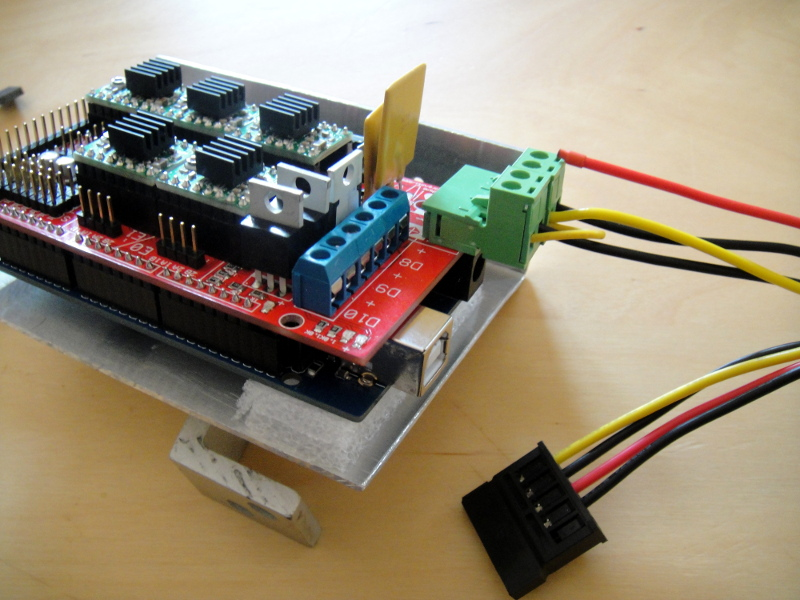
\includegraphics[width=10cm]{img/ramps02.jpg}}%
\end{figure}%
\subsubsection{Alimentation externe} %
Il faut maintenant l'alimentation externe sur la RAMPS (bornier vert à quatre broches). %
Il est préconisé d'alimenter en 12V. J'ai donc utilisé une alimentation de PC (500W, %
qui peut le plus, peu le moins). Pour info, le 0V, c'est le fil noir, le 12V, c'est le %
fil jaune. Comme d'habitude, l'alimentation de PC est un élément que j'ai trouvé %
dans un vide-grenier (5\euro{}). Il y a une entrée 5A et une entrée 11A. Mon %
alimentation a une capacité de 18A sur la sortie 12V. Il m'a donc suffit de mettre %
les deux entrées en parallèle sur le 12V fig. \ref{alimentation} %
page~\pageref{alimentation}).%
\begin{figure}%
   \caption{\label{alimentation} Branchement de l'alimentation externe}%
   \center{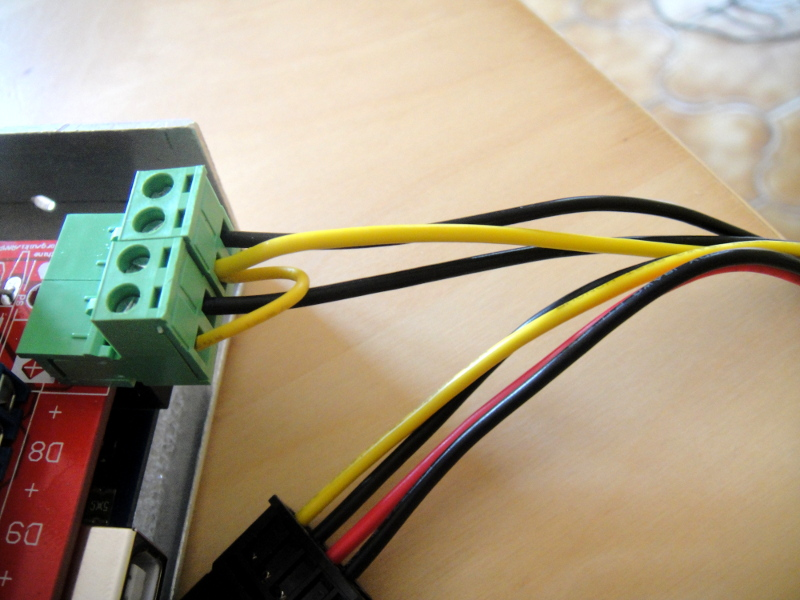
\includegraphics[width=10cm]{img/ramps03.jpg}}%
\end{figure}%
\subsubsection{Les premières embuches}
Ce qui devait arriver arriva. En faisant des essais sur la carte RAMPS, j'ai fait un %
court-circuit (5v relié au 0V). Une seconde a suffit pour que de la fumée s'échappe %
de la Funduino. Une %
fois l'ensemble démonté, un composant avait pris copieux. \par %
Diagnostique : quand je branche seul, le Funduino au PC avec le cordon USB, le %
périphérique est reconnu. Si maintenant, j'alimente la RAMPS en 12V, le PC perd la %
connection USB. C'est embêtant. Dans ces cas là, il faut garder son calme. La %
Funduino, tout comme l'Arduino est une carte super simple : il y a un micro controlleur, %
quelques résistances, un condensateur, parfois une interface USB (sinon, pris en charge %
par le micro controlleur), et ... un régulateur de tension (AMS1117). Ce régulateur de %
tension permet de garder 5V dans le circuit quelque soit la tension d'alimentation (tant %
qu'elle reste au dessus de 5V). C'est un composant à trois pattes équipé d'un radiateur, qui %
ressemble à une quatrième patte (fig. \ref{regulator} page~\pageref{regulator}). %
\begin{figure}%
   \caption{\label{regulator} Régulateurs de tension}%
   \center{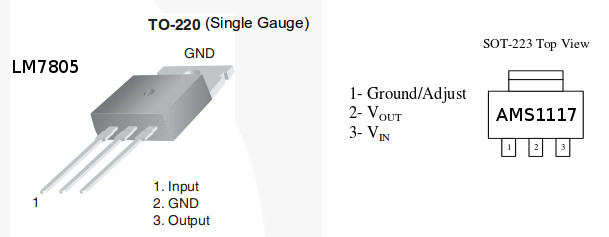
\includegraphics[width=10cm]{img/regulator.jpg}}%
\end{figure}%
\begin{figure}%
   \caption{\label{arduino_principle} Schéma de principe du Funduino}%
   \center{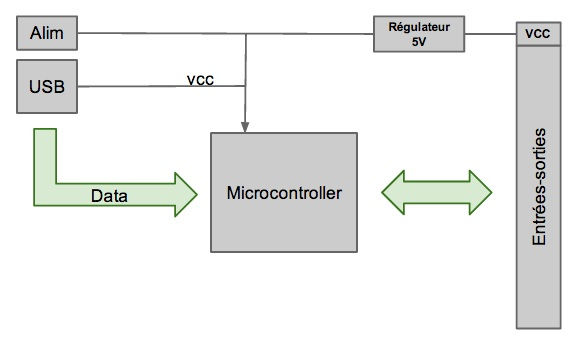
\includegraphics[width=10cm]{img/arduino_principle.jpg}}%
\end{figure}%
En regardant bien, c'est ce composant qui a chargé. %
En regardant le schéma de la figure \ref{arduino_principle} en page~\pageref{arduino_principle}, %
on comprend bien pourquoi le Funduino fonctionnait avec l'alimentation USB, et ne %
fonctionnait plus avec une alimentation externe. \par%
La réparation est simple : le LM7805 rempli la même fonction. Il est carrément plus gros, %
mais, on va trouver à le loger. J'en ai un sous le coude, c'est parti. Il faut être %
vigilent sur l'ordre des pattes. Pour s'adapter au circuit, il faut croiser le OUT %
et le GND pour avoir dans l'ordre [IN OUT GND] (fig. \ref{regulator} page~\pageref{regulator}). Ensuite on soude (fig. \ref{funduino_repared} %
page~\pageref{funduino_repared}). J'ai pris soin de mettre un scotch sur le radiateur du %
LM7805 pour éviter que la partie métallique ne touche une autre partie de la Funduino.\par{} %
Je rebranche le tout, et ... c'est reparti comme en 40 ! Ce qu'il faut retenir, c'est %
que la Funduino est très fragile (en même temps, un court-circuit ne pardonne pas), %
et qu'il faut vérifier à deux fois avant de brancher quelque chose (on ne branchera %
rien à chaud !).%
\begin{figure}%
   \caption{\label{funduino_repared} Funduino avec son nouveau régulateur de tension}%
   \center{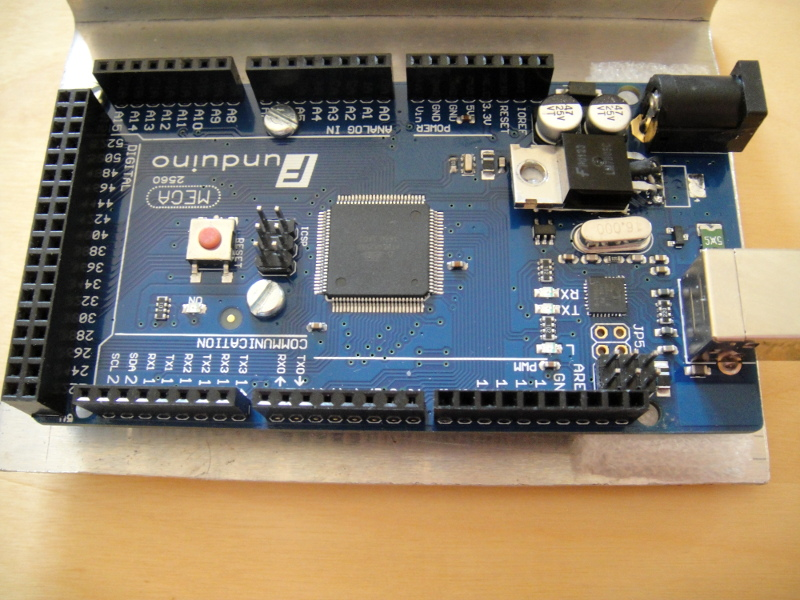
\includegraphics[width=10cm]{img/funduino02.jpg}}%
\end{figure}%
\subsection{Réglage des controlleurs de moteurs}
\subsubsection{Principe du réglage}
Vous avez dû remarquer que sur chaque contrôleur A4988, il y a un potentiomètre. Il sert %
à quelque chose. En fait, le composant A4988 est pourvu d'un régulateur de courant. \c{C}a tombe %
bien, les moteurs que j'ai achetés (42BYGHW609) ont un ampérage maximum de 1,7A. Nous allons %
donc agir sur ce potentiomètre pour que l'intensité de sortie ne dépasse pas 1,7A.
\subsubsection{Câblage du module}
Nous allons faire un petit banc de test pour régler nos modules (fig. \ref{a4988_wired} %
page~\pageref{a4988_wired}). Procédez ainsi:\begin{dinglist}{71}%
\item{Branchez GND sur le 0V de l'Arduino}%
\item{Branchez VDD sur le 5V de l'Arduino}%
\item{Branchez /RESET et /SLEEP sur 5V}
\item{Branchez /ENABLE sur la pin 13 de l'Arduino}
\item{Branchez STEP sur la pin 12 de l'Arduino}
\item{Branchez DIR sur la pin 11 de l'Arduino}
\item{Branchez VMOT sur le 12V de l'alimentation externe (alimentation d'ordinateur)}
\item{Branchez un bobinage moteur sur 1A, 1B}
\item{Branchez l'autre bobinage moteur sur 2A, 2B}
\end{dinglist}%
Pour trouver un bobinage moteur, sans alimentation, reliez deux broches du moteur et tounez l'axe %
à la main; s'il y a une petite résistance à la rotation, c'est que vous avez courcircuité un bobinage %
(c'est dû aux courants de Foucault). Sinon, testez une autre paire%
\begin{figure}%
   \caption{\label{a4988_wired} câblage du A4988}%
   \center{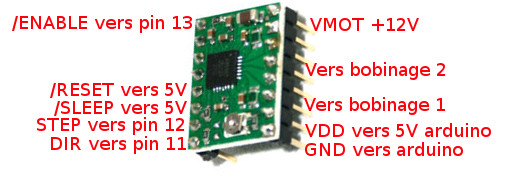
\includegraphics[width=10cm]{img/a4988_1.jpg}}%
\end{figure}%
\subsubsection{Le test}
Insésez un ampèremètre dans le circuit d'un bobinage (l'ampèremètre se branche en série), et chargez %
le programme suivant dans l'arduino:
\begin{verbatim}
/*
Test moteur PAP (pas entier)
Carte Pololu avec puce A4988 + régulateur de tension > 
http://www.pololu.com/catalog/product/1183
Ch.Aubert Déc.2011
*/

/************** Définition des E/S *************************/
const int dirPin = 11;  // DIR
const int stepPin = 12; // STEP
const int enablePin = 13; // ENABLE

void setup()
{
  pinMode(stepPin, OUTPUT); // Dir et Step en sortie
  pinMode(dirPin, OUTPUT);
  pinMode(enablePin, OUTPUT); // broche Enable en sortie
  digitalWrite(enablePin, HIGH);

  calibrate(); // lance le stall moteur Ampérage max !
  //test(); // lance le test !!
}

void loop()
{
  // rien pour l'instant !
}

void calibrate() // Stall moteur Ampérage max !
{
  digitalWrite(enablePin, LOW);
}

void test() //  faire tourner le moteur 200 pas
{
  int j;
  digitalWrite(enablePin, LOW);
  delayMicroseconds(2);

  digitalWrite(dirPin, HIGH);
  for(j=0; j<=199; j++) {
    delay(200);
    digitalWrite(stepPin, LOW);
    delayMicroseconds(10);
    digitalWrite(stepPin, HIGH);
    delayMicroseconds(1000);
  }
  digitalWrite(enablePin, HIGH); 
}
\end{verbatim}
\begin{figure}%
   \caption{\label{a4988_montage} câblage du A4988}%
   \center{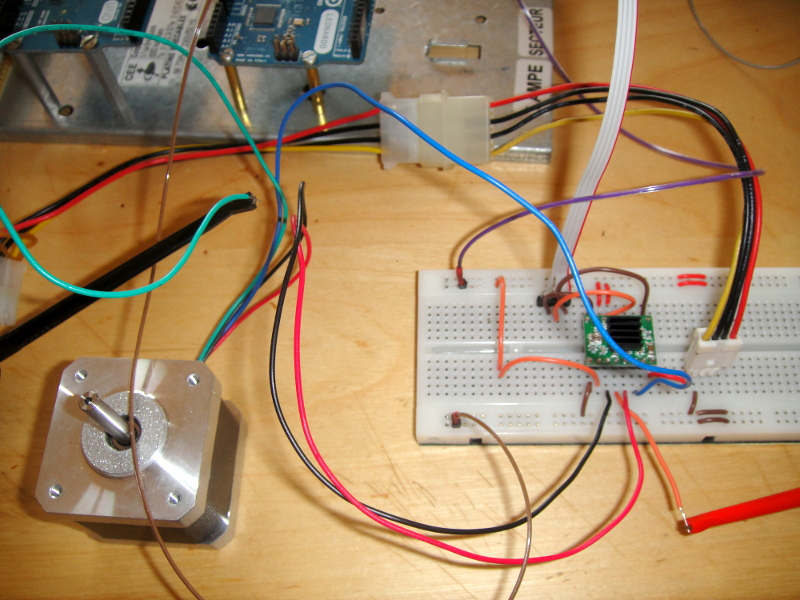
\includegraphics[width=10cm]{img/montage_a4988.jpg}}%
\end{figure}%
\begin{figure}%
   \caption{\label{a4988_ampere} câblage du A4988}%
   \center{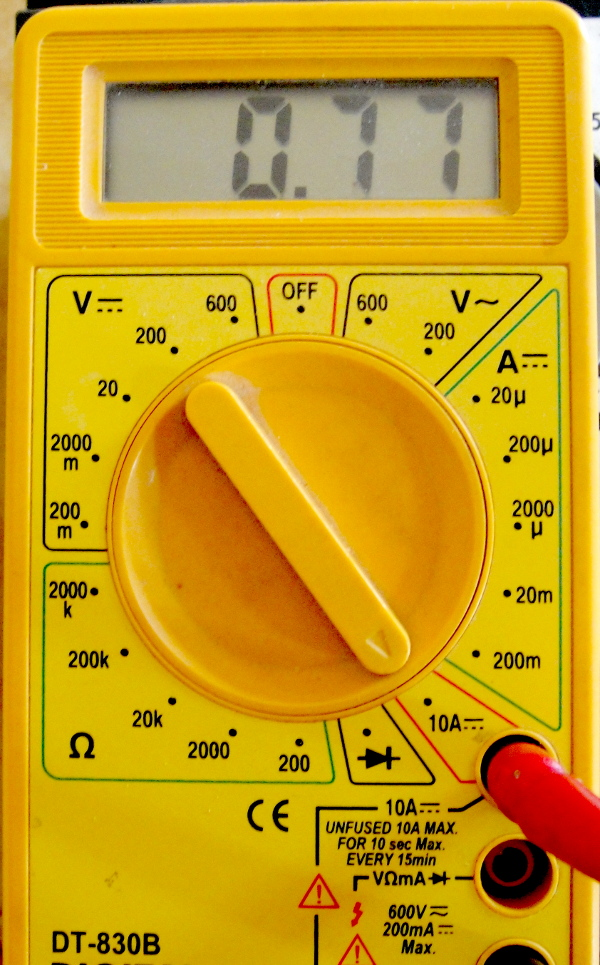
\includegraphics[width=5cm]{img/amperemetre.jpg}}%
\end{figure}%
Alimentez l'arduino (par le cable USB), et branchez l'alimentation. Attention, on ne décâble jamais %
le moteur lorsque les alimentations (arduino et alim externe de 12V) sont en marche. Par l'effet de %
courants induits, un retour de courant pourrait détruire votre contrôleur. Normalement, le moteur %
ne tourne pas, mais l'axe est rigide. \\%
N'utilisez pas de tournevis à manche métalique; j'ai remarqué que les mesures sont faussées. Tournez le %
potentiomètre pour ne pas dépasser 0,7 courant max (1,2A pour ma part). J'ai fait le choix de brider %
à 0,8A (fig. \ref{a4988_ampere} page~\pageref{a4988_ampere}). %